%------------------------------------------------
\section{Hyperparameter tuning}
%------------------------------------------------
\begin{frame}[t]
	\frametitle{Hyperparameter tuning}
	\tikzstyle{background grid}=[draw, black!50,step=.5cm]
	%
	We can use StoMADS to tune the hyperparameters \ifshowcitations\footpartcite{Khalil2021}\fi\\
	%
	\tikzstyle{background grid}=[draw, black!50,step=.5cm]
	\begin{tikzpicture}[remember picture, overlay] %show background grid, 
		% Put the graphic inside a node. This makes it easy to place the
		% graphic and to draw on top of it. 
		% The above right option is used to place the lower left corner
		% of the image at the (0,0) coordinate. 
		\node [inner sep=0pt,above right, opacity=1.0]  at (-0.01\textwidth,-0.7\textheight) (error) 
			{
				\only<1>{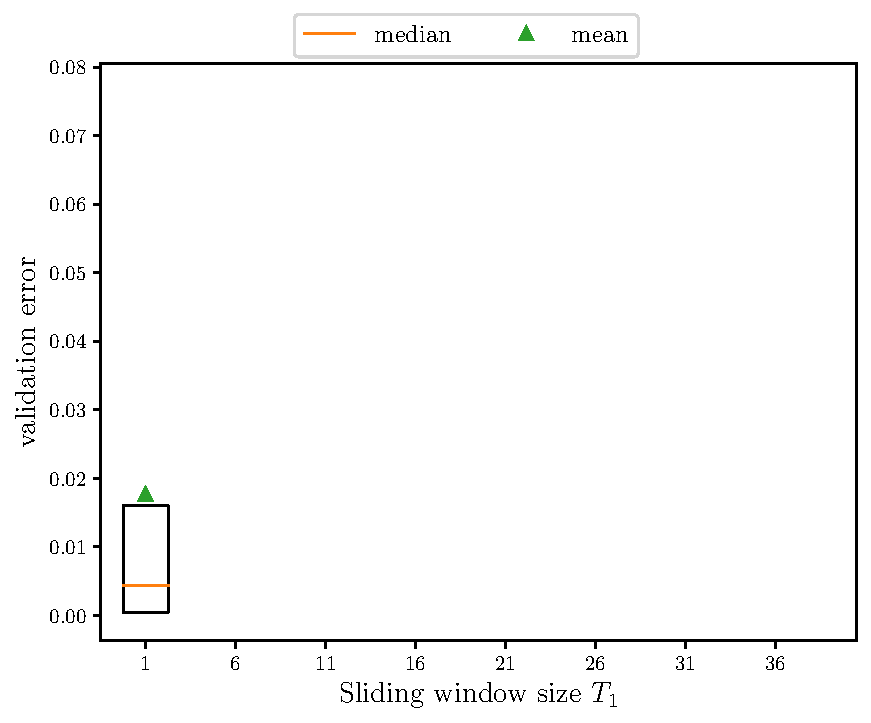
\includegraphics[width=0.5\textwidth]{box_plots/boxplot_input_dim_0.pdf}}%
				\only<2>{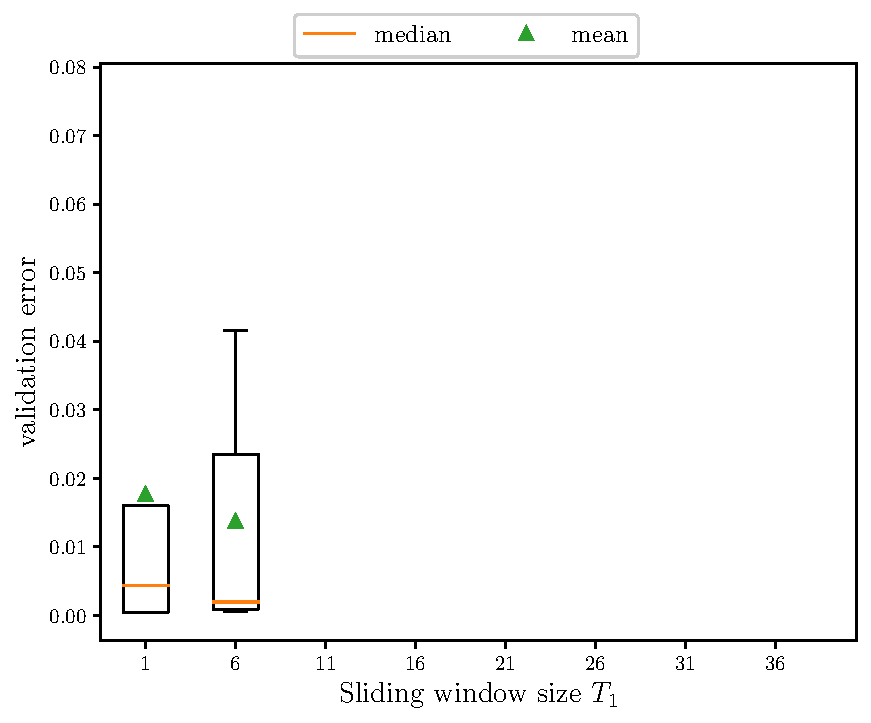
\includegraphics[width=0.5\textwidth]{box_plots/boxplot_input_dim_1.pdf}}%
				\only<3>{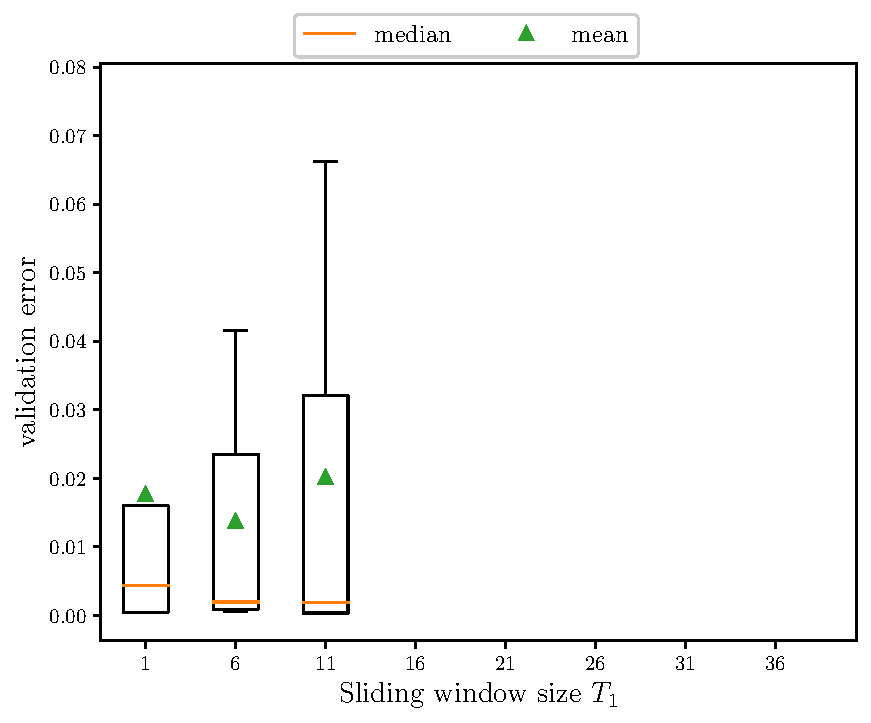
\includegraphics[width=0.5\textwidth]{box_plots/boxplot_input_dim_2.pdf}}%
				\only<4>{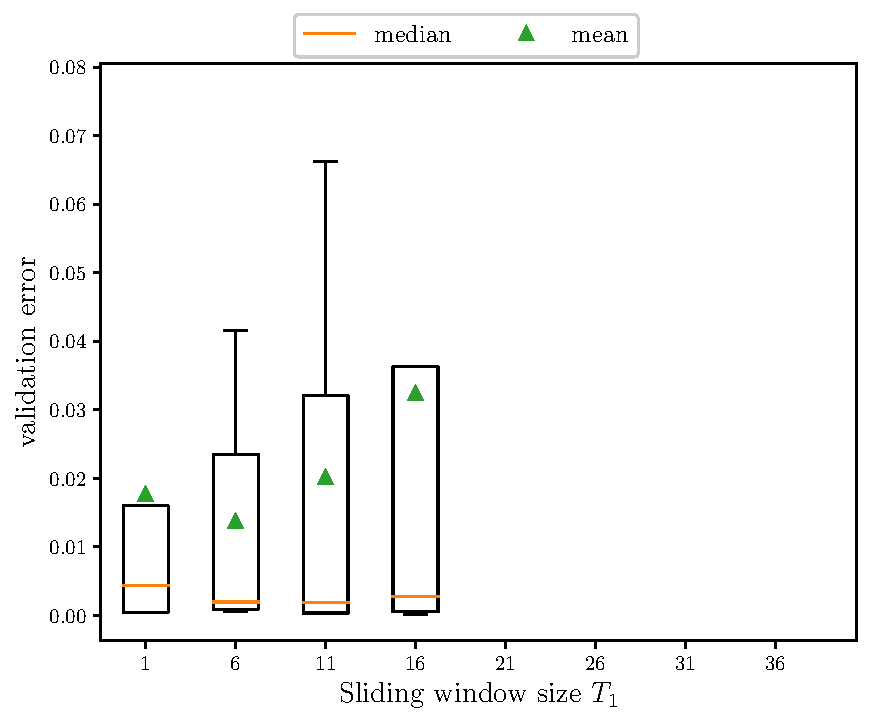
\includegraphics[width=0.5\textwidth]{box_plots/boxplot_input_dim_3.pdf}}%
				\only<5>{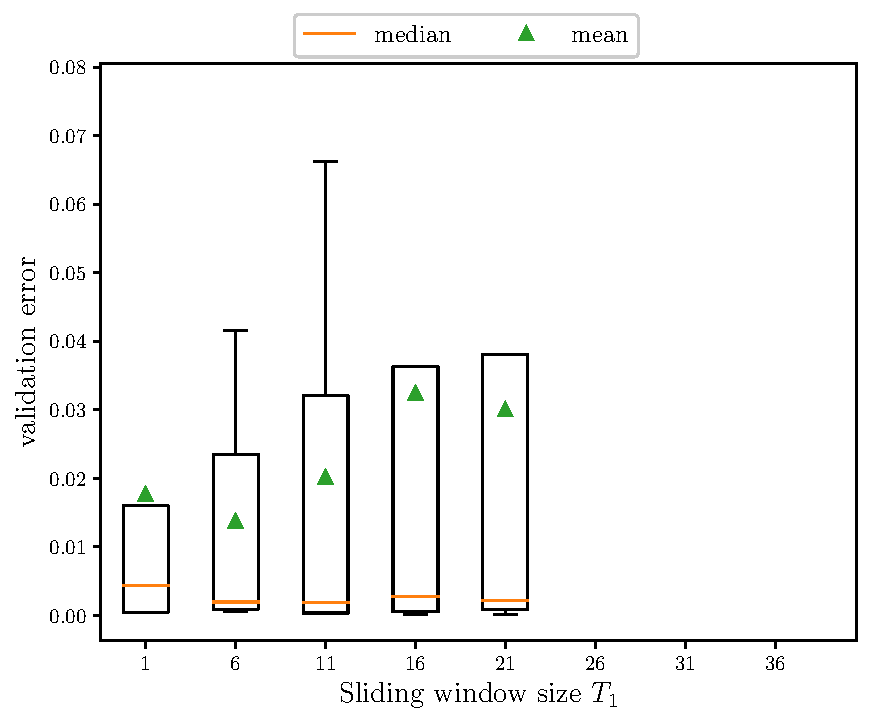
\includegraphics[width=0.5\textwidth]{box_plots/boxplot_input_dim_4.pdf}}%
				\only<6>{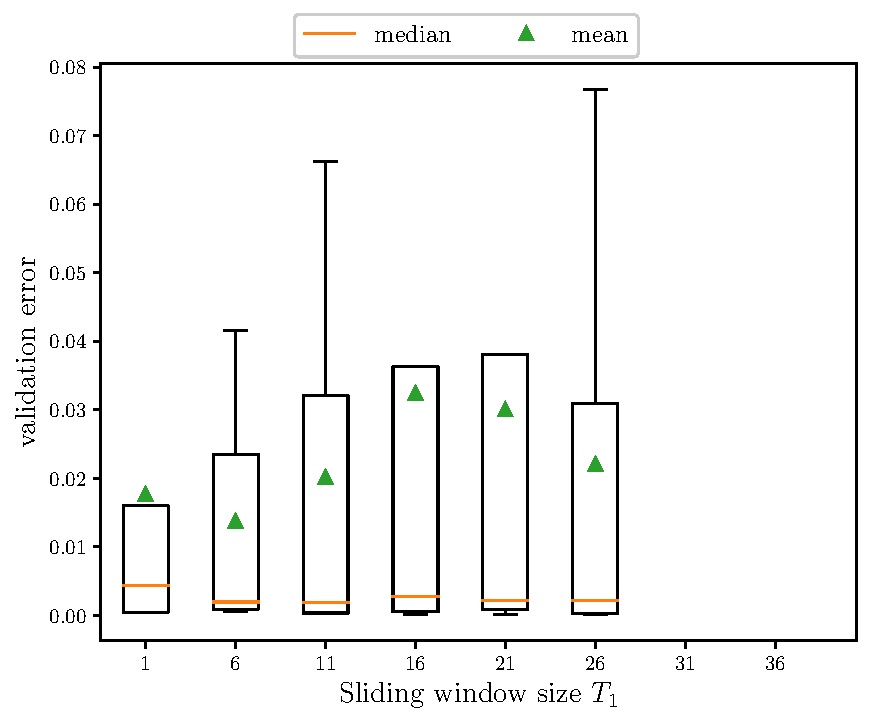
\includegraphics[width=0.5\textwidth]{box_plots/boxplot_input_dim_5.pdf}}%
				\only<7>{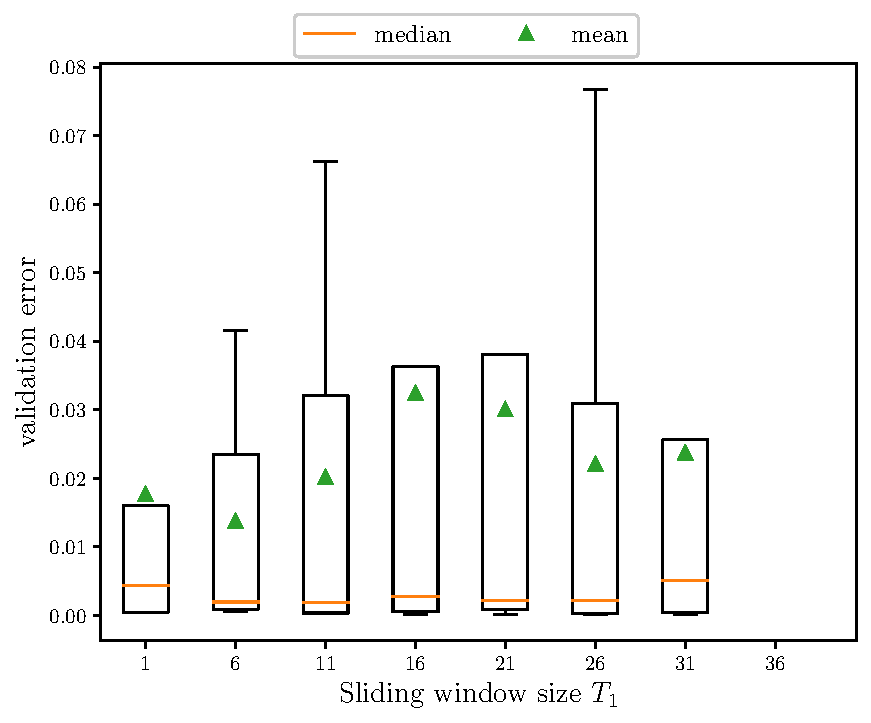
\includegraphics[width=0.5\textwidth]{box_plots/boxplot_input_dim_6.pdf}}%
				\only<8>{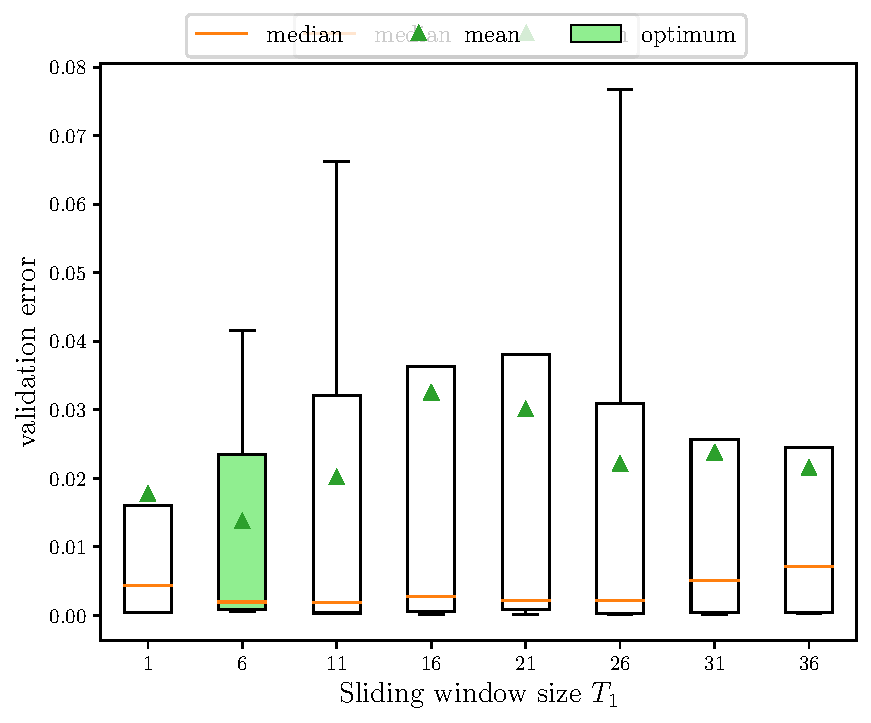
\includegraphics[width=0.5\textwidth]{box_plots/boxplot_input_dim_opt.pdf}}%
				\only<9>{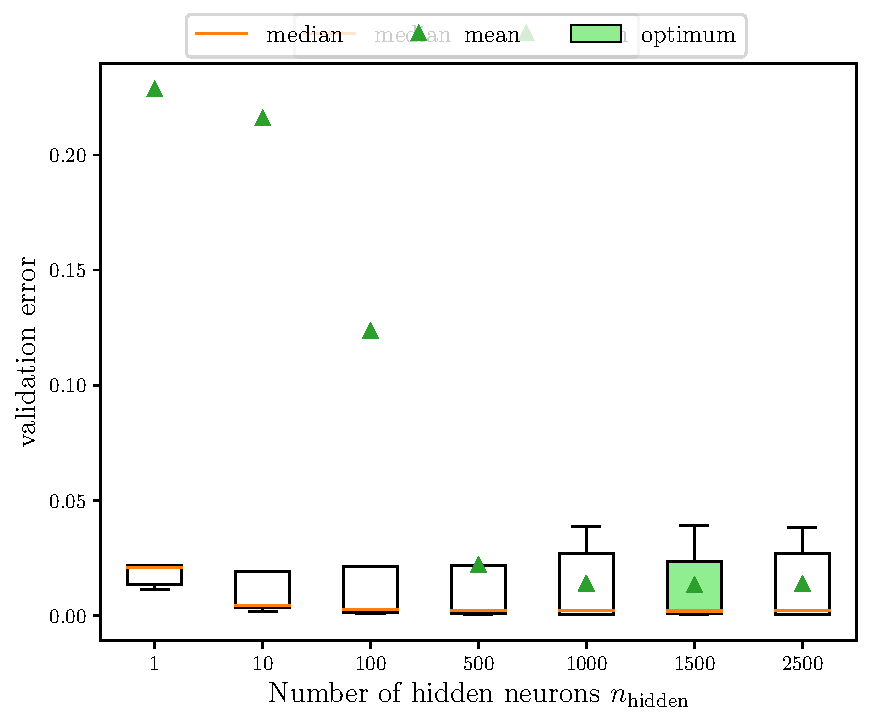
\includegraphics[width=0.5\textwidth]{box_plots/boxplot_hid_dim_opt.pdf}}%
				\only<10>{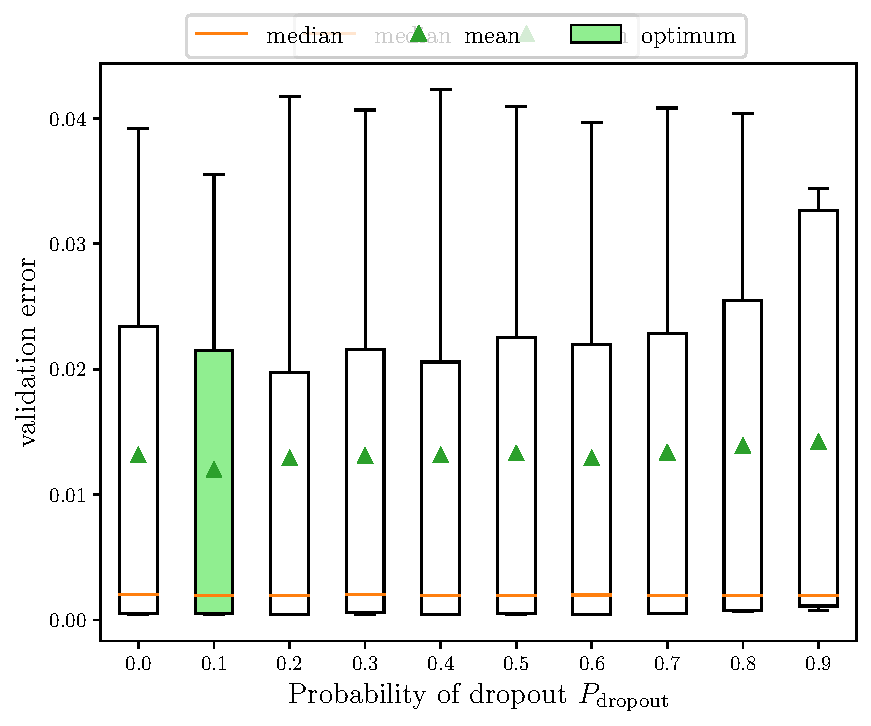
\includegraphics[width=0.5\textwidth]{box_plots/boxplot_dropout_opt.pdf}}%
			};
		\node [inner sep=0pt,above left, opacity=1.0]  at (1.01\textwidth,-0.7\textheight) (prediction) 
			{
				\only<1>{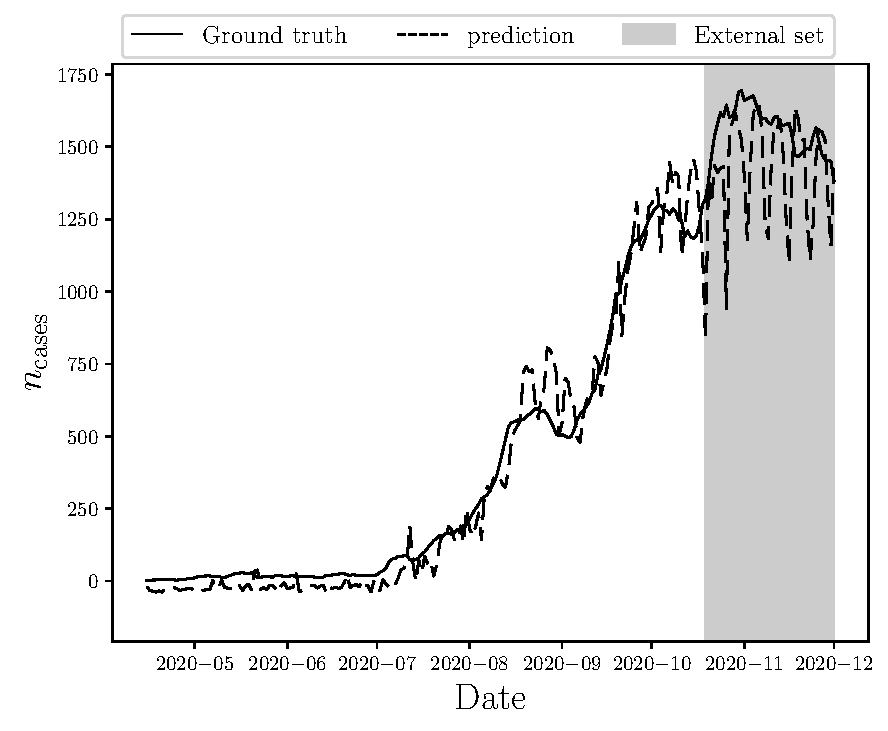
\includegraphics[width=0.5\textwidth]{models/model_input_dim_0.pdf}}%
				\only<2>{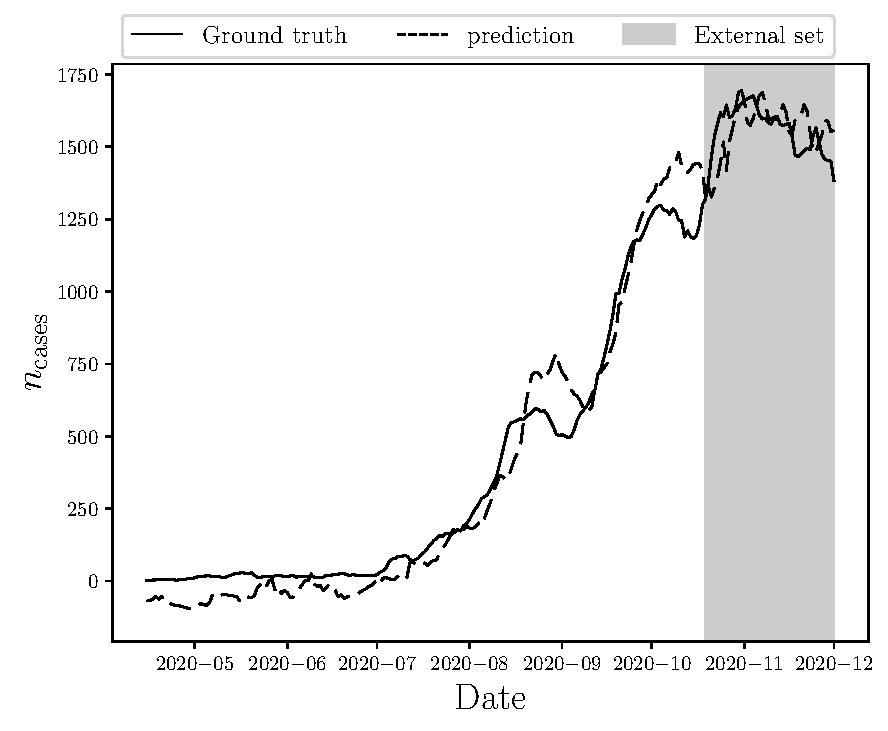
\includegraphics[width=0.5\textwidth]{models/model_input_dim_1.pdf}}%
				\only<3>{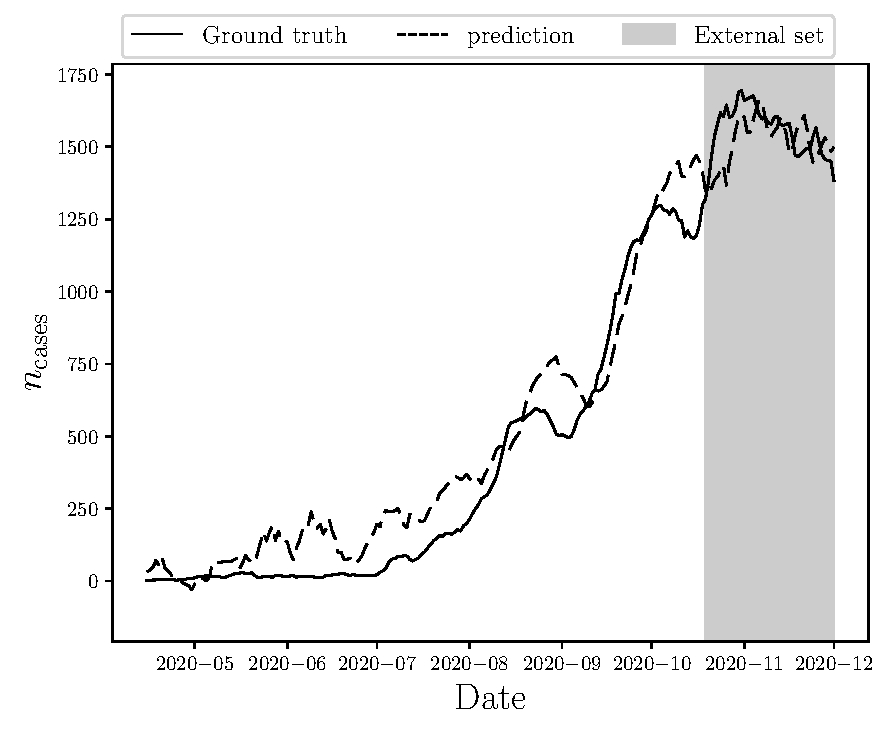
\includegraphics[width=0.5\textwidth]{models/model_input_dim_2.pdf}}%
				\only<4>{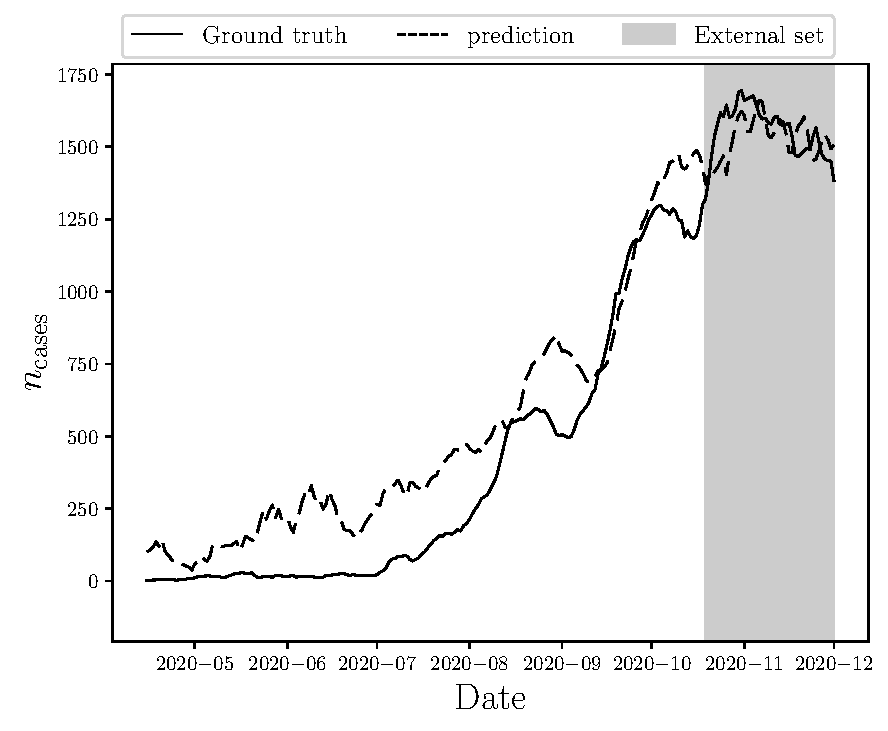
\includegraphics[width=0.5\textwidth]{models/model_input_dim_3.pdf}}%
				\only<5>{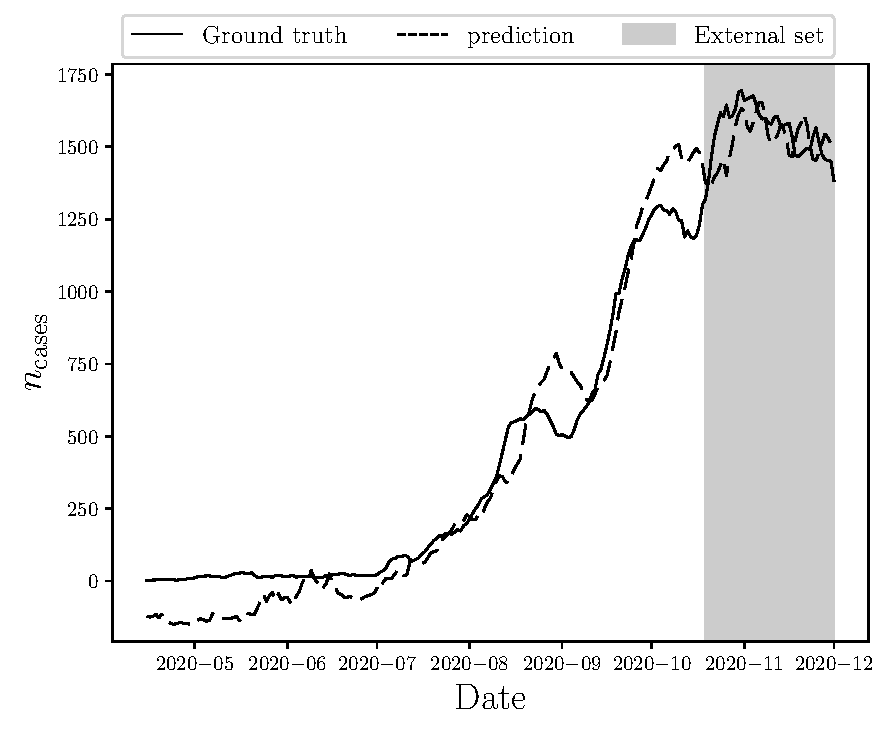
\includegraphics[width=0.5\textwidth]{models/model_input_dim_4.pdf}}%
				\only<6>{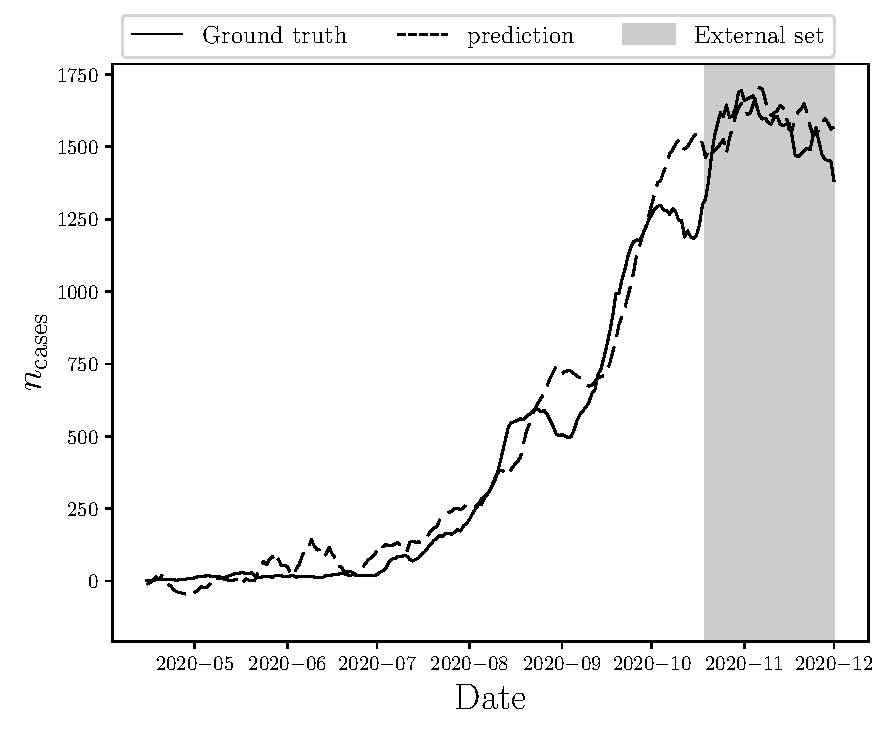
\includegraphics[width=0.5\textwidth]{models/model_input_dim_5.pdf}}%
				\only<7>{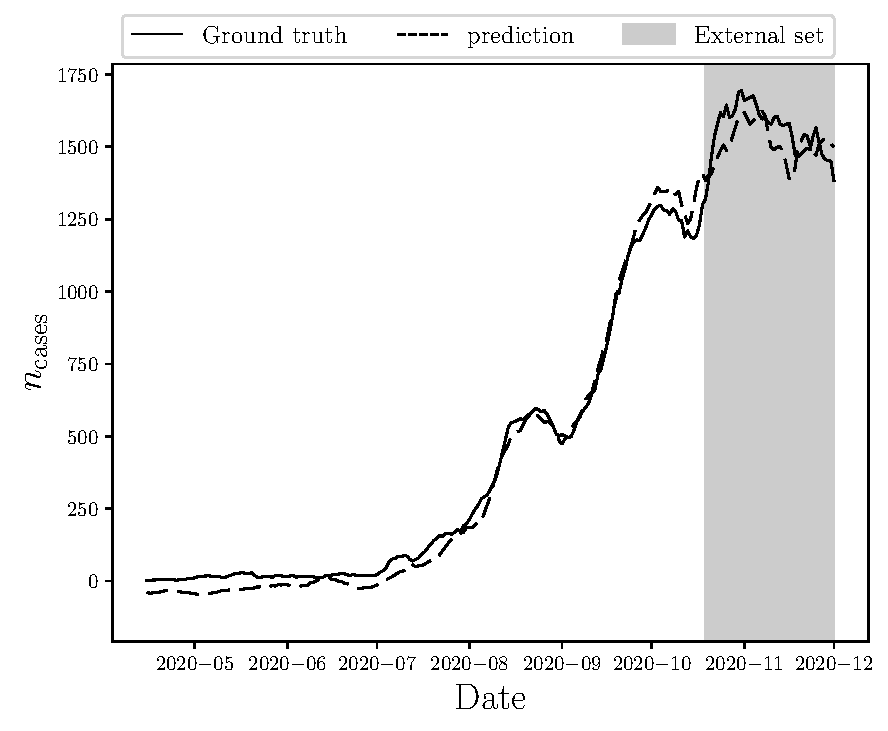
\includegraphics[width=0.5\textwidth]{models/model_input_dim_6.pdf}}%
				\only<8>{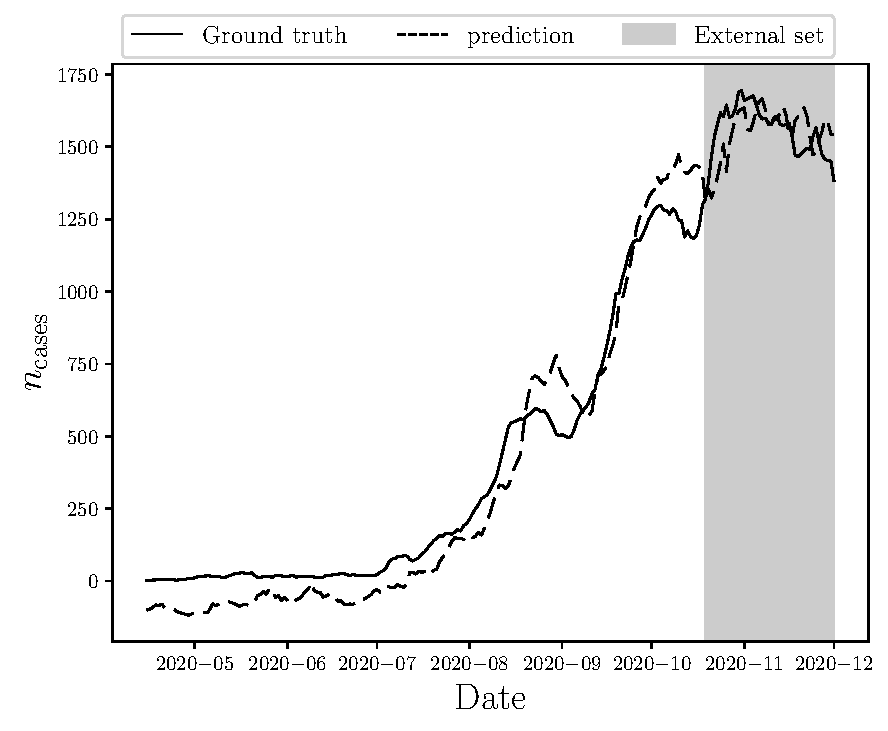
\includegraphics[width=0.5\textwidth]{models/final_model_input_dim.pdf}}%
				\only<9>{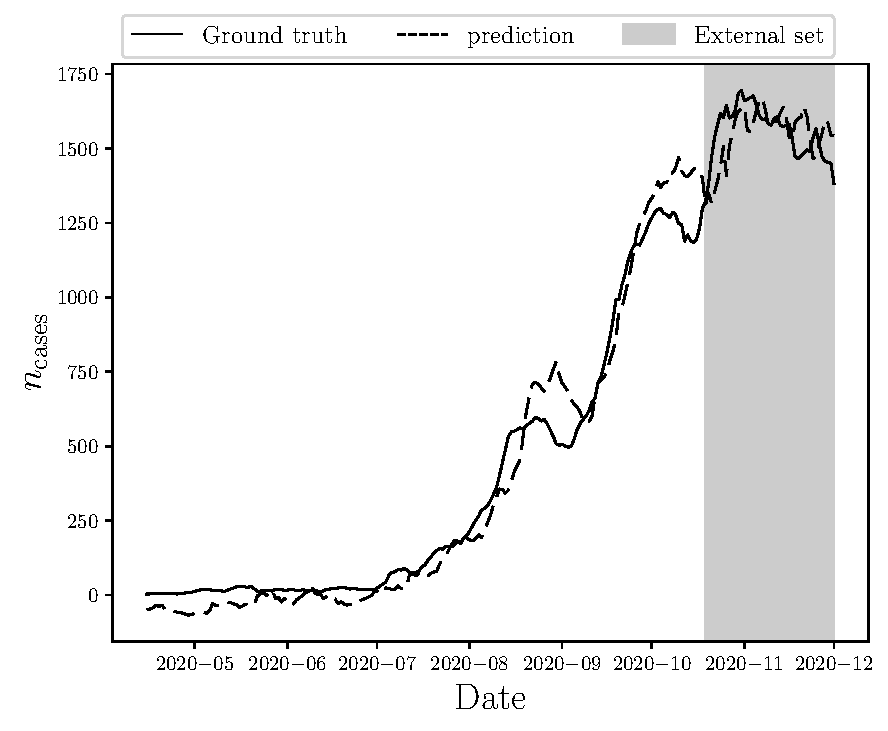
\includegraphics[width=0.5\textwidth]{models/final_model_hid_dim.pdf}}%
				\only<10->{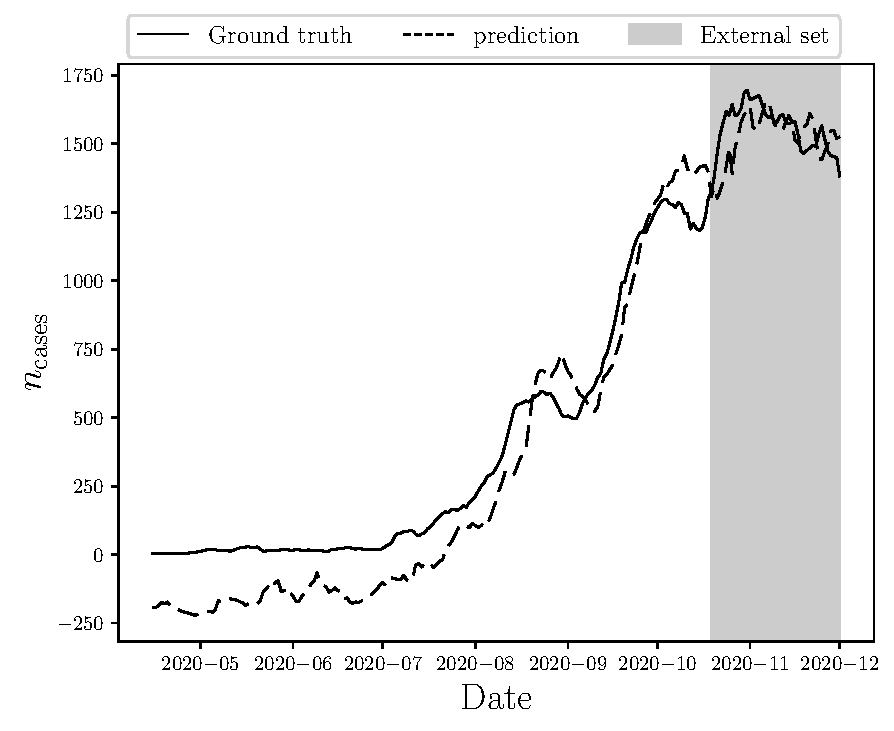
\includegraphics[width=0.5\textwidth]{models/final_model_dropout.pdf}}%
			};
		% show origin
		% \fill (0,0) circle (2pt);
	\end{tikzpicture}%
	%
	\begin{columns}[t] % The "c" option specifies centered vertical alignment while the "t" option is used for top vertical alignment
		\begin{column}{.42\textwidth} % Left column and width
			\vspace{-2.0em}
			% Optimization problem
			\uncover<11->{
				\begin{exampleblock}{Objective and constraints}
					\vspace{-0.0em}
					\begin{equation*}
						\begin{aligned}
							& \underset{\mathbf{x}}{\text{min}}
							& & f(\mathbf{x}) = \mathbb{E}_{\Theta}\left[{f}_{\Theta}(\mathbf{x}) = \mathrm{error}_\mathrm{CV}\right]\\
							& \text{where}
							& & \Theta\mathrm{:realizations}
						\end{aligned}
					\end{equation*}
				\end{exampleblock}
			}%
			\vspace{-0.5em}
			\uncover<11->{
				% Variables
				\begin{alertblock}{Design variables ($\mathbf{x}$)}
					\vspace{-0.0em}
						\begin{itemize}\itemsep0em
							\item $T_1:$ Input dimension
							\item $n_\text{hidden}:$ Number of hidden neurons
							\item $P_\text{dropout}:$ Probability of dropout, etc.
						\end{itemize}
				\end{alertblock}
			}%
			\vspace{-0.5em}
			\uncover<11->{
				% Parameters
				\begin{blueblock}{Randomly seeded parameters}
					\vspace{-0.0em}
					\begin{itemize}\itemsep0em
						\item Initial weights
						\item Gradient descent steps
					\end{itemize}
				\end{blueblock}
			}%
		\end{column}
		%
		\begin{column}{.5\textwidth} % Left column and width
		\end{column}
	
	\end{columns}
	%
	\vspace{-3em}
\end{frame}
\addtocounter{footnote}{-1}
%------------------------------------------------